\documentclass[tikz,border=10pt]{standalone}
\usepackage{amsmath}
\usepackage{amssymb}

\usetikzlibrary{arrows.meta, positioning, calc}

\begin{document}

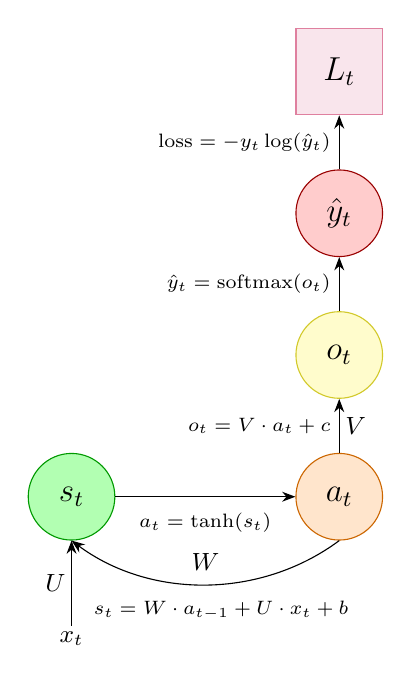
\begin{tikzpicture}[
    >=Stealth,
    % Define styles matching your original layout
    s_node/.style={circle, draw=green!60!black, fill=green!30, minimum size=1.1cm, font=\large},
    a_node/.style={circle, draw=orange!80!black, fill=orange!20, minimum size=1.1cm, font=\large},
    o_node/.style={circle, draw=yellow!80!black, fill=yellow!20, minimum size=1.1cm, font=\large},
    y_node/.style={circle, draw=red!60!black, fill=red!20, minimum size=1.1cm, font=\large},
    loss_node/.style={rectangle, draw=purple!50, fill=purple!10, minimum size=1.1cm, font=\large},
    lbl/.style={font=\small, inner sep=2pt},
    math_lbl/.style={font=\scriptsize, inner sep=3pt} 
]

    % --- Single Column Nodes (Time Step t) ---
    \node[s_node] (s) at (0,0) {$s_{t}$};
    \node[a_node] (a) at ($(s) + (3.4, 0)$) {$a_{t}$}; 
    \node[lbl] (x) at ($(s) + (0, -1.8)$) {$x_{t}$};
    
    \node[o_node] (o) at ($(a) + (0, 1.8)$) {$o_{t}$};
    \node[y_node] (y) at ($(o) + (0, 1.8)$) {$\hat{y}_{t}$};
    \node[loss_node] (L) at ($(y) + (0, 1.8)$) {$L_{t}$};
    
    % --- Vertical and Internal Column Flows ---
    \draw[->] (x) -- node[left, lbl] {$U$} (s);
    \draw[->] (s) -- node[below, math_lbl, yshift=-1mm] {$a_{t} = \tanh(s_{t})$} (a);
    \draw[->] (a) -- node[right, lbl] {$V$} node[left, math_lbl] {$o_{t} = V \cdot a_{t} + c$} (o);
    \draw[->] (o) -- node[left, math_lbl] {$\hat{y}_{t} = \text{softmax}(o_{t})$} (y);
    \draw[->] (y) -- node[left, math_lbl] {$\text{loss} = -y_{t}\log(\hat{y}_{t})$} (L);

% --- Recurrent Feedback Loop (W Matrix) ---
    % Routes a path exiting the bottom of a_t, looping backwards underneath,
    % and entering the bottom of s_t.
    \draw[->] (a.south) .. controls ($(a) + (-1.0, -1.3)$) and ($(s) + (1.0, -1.3)$) .. 
        node[below, math_lbl, yshift=-1mm,xshift=2mm] {$s_t = W \cdot a_{t-1} + U \cdot x_t + b$} 
        node[above, lbl, yshift=1mm] {$W$} (s.south);

\end{tikzpicture}
\end{document}